\chapter{Operations and Logistics}
\label{ch:Operations_and_Logistics}
The logistics and operations involved in designing and managing an autonomous eVTOL fleet are extensive.
Monitoring the vehicles, their environments, such as Air Traffic Control (ATC) and vertiports operations, requires Remote Operations Centres (ROCs).
These ROCs will stay crucial to monitor fleet operations, address emergencies, and, most importantly, ensure safety.
This chapter analyses the vertiports operations and logistics in \Cref{sec:vertiport_logistic}, and conducts a Reliability, Availability, Maintainability and Safety (RAMS) analysis in \Cref{sec:Reliability_Availability_Maintainability_and_Safety}.

\section{Vertiports}
\label{sec:vertiport_logistic}
Due to the versatility of the \textit{Swing} design, many different vertiport configurations are possible.
As earlier stated in the Market Analysis (\Cref{ch:Market_Analysis}), there are three main vertiport configurations: vertistops, vertihubs, and vertibases.
All three are different in size, services, and placement; however, there are even more possible configurations, as can be seen from \Cref{fig:lilium_vertiport_sizing,fig:eas_vertiport}
These differences account for specific operations and logistics, which would be too extensive for the scope of this report; hence, the following paragraph will discuss the three typical configurations split up into flight scheduling, pre-flight, take-off, in-flight, approach and landing, and post-flight \cite{boeing2021conops}.

\begin{minipage}{0.65\linewidth}
    \begin{figure}[H]
    \centering
    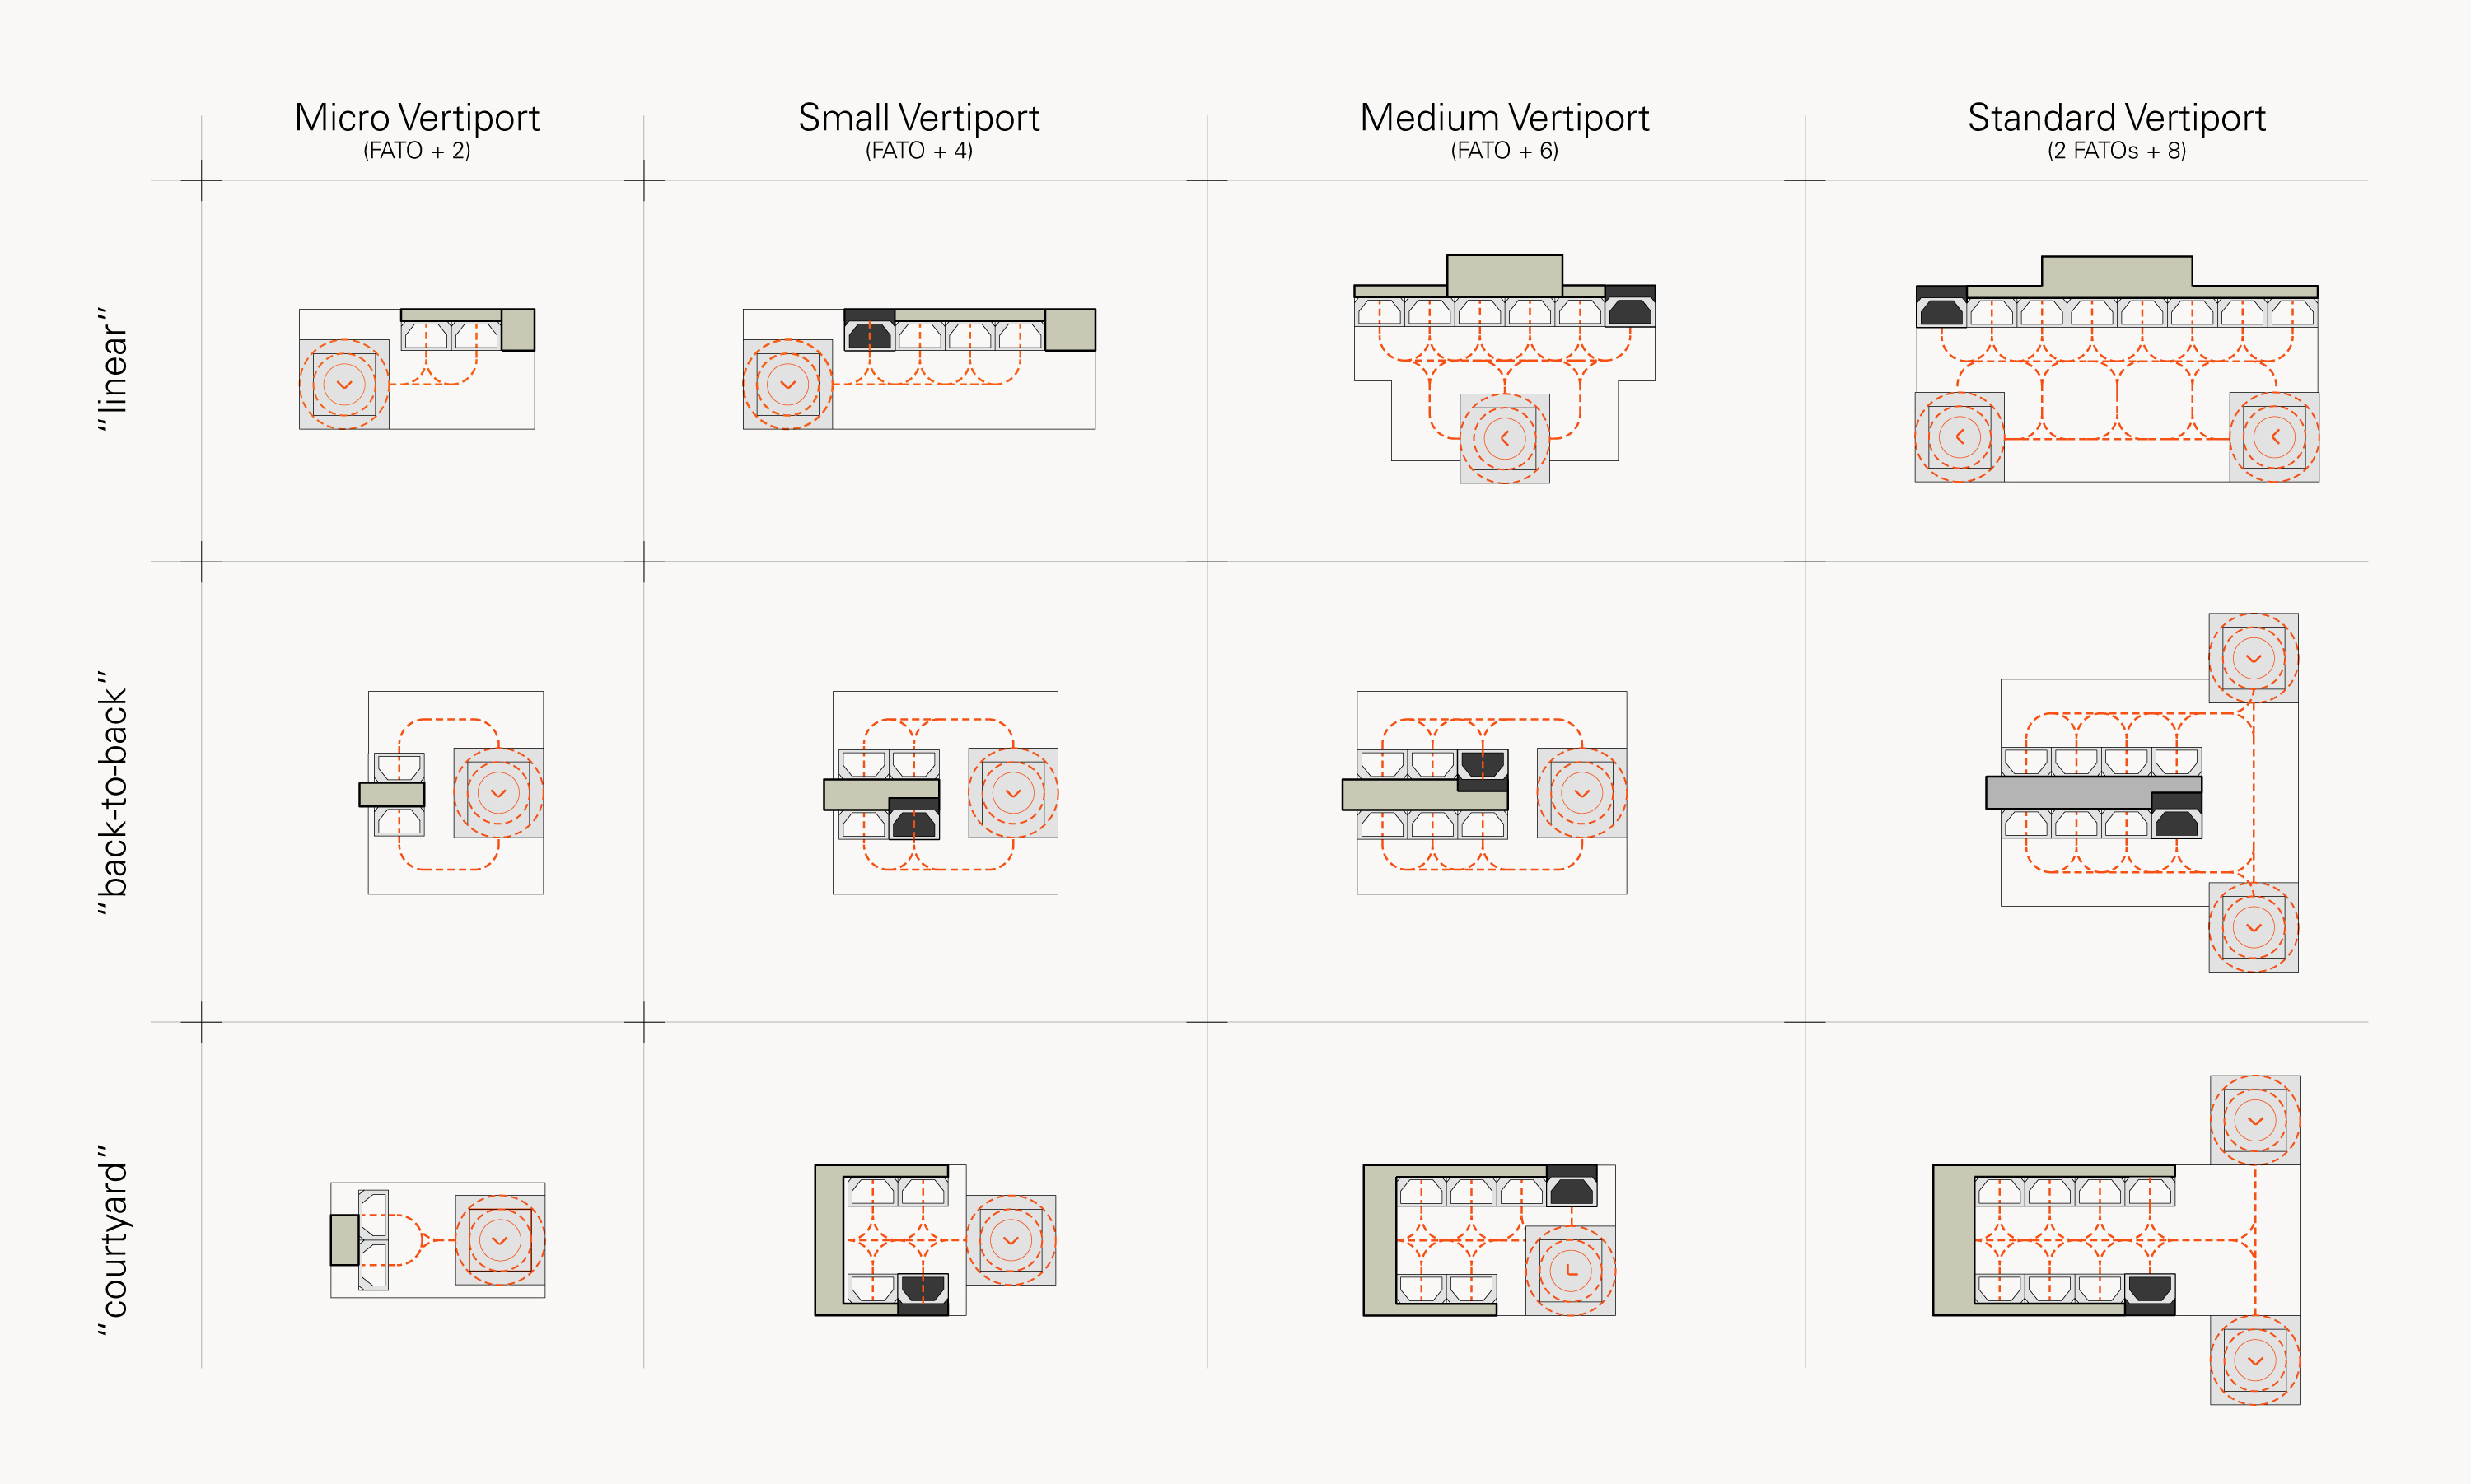
\includegraphics[width=1\linewidth]{figures/lilium vertiport configs}
    \caption{Lilium vertiport sizing \cite{lilium2020designvertiports}}
    \label{fig:lilium_vertiport_sizing}
    \end{figure}
\end{minipage}
\begin{minipage}{0.35\linewidth}
    \begin{figure}[H]
    \centering
    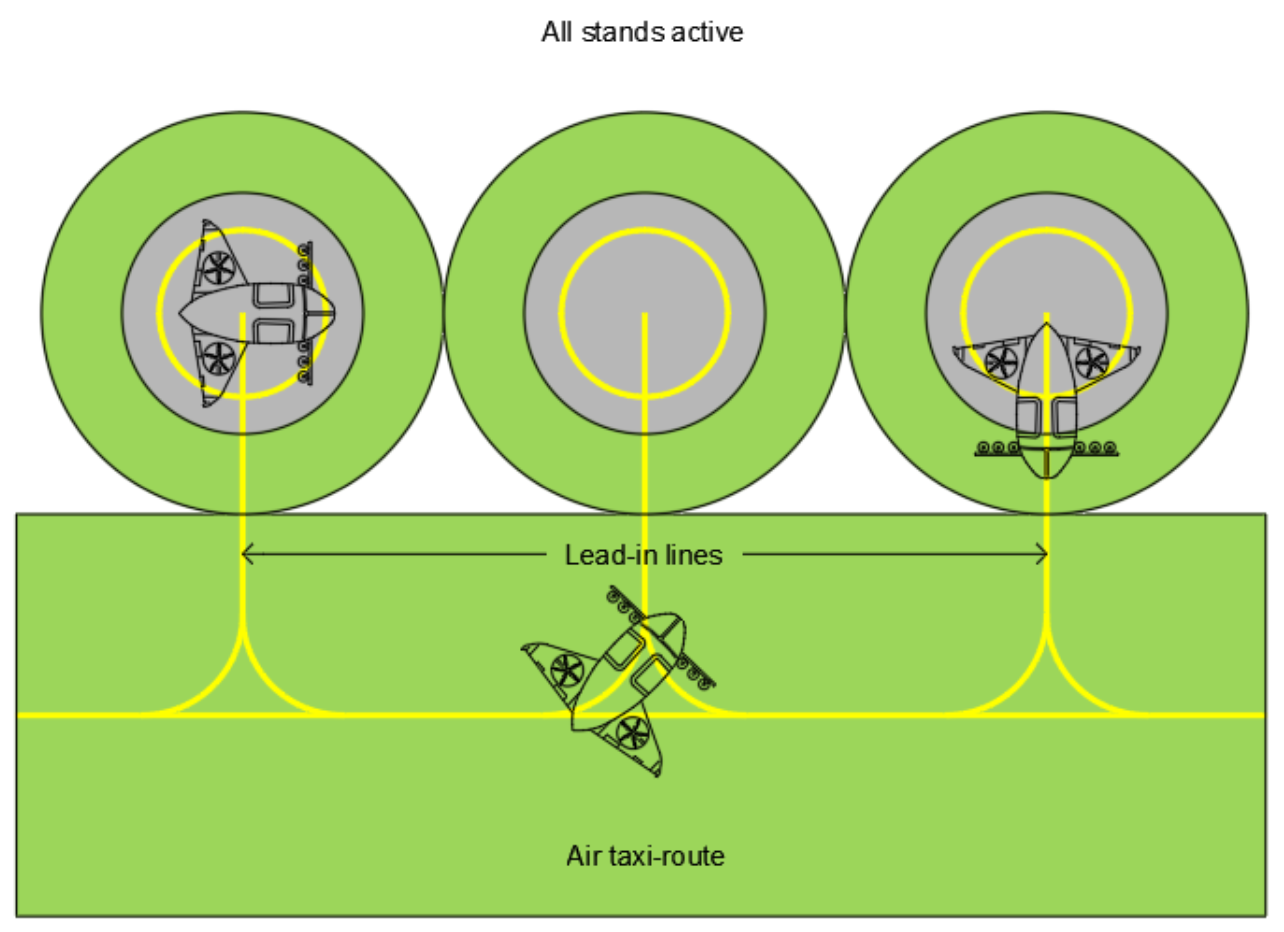
\includegraphics[width=1\linewidth]{figures/Vertiport_easa}
    \caption{EASA vertiport concept \cite{easa2022vertiports}}
    \label{fig:eas_vertiport}
    \end{figure}
\end{minipage}

\subsubsection{Flight Scheduling}
The flight scheduling starts when the ROC receives demand forecasts for flights between vertiports.
The operator sets the mission up and checks with ATC and the vertiport for a time slot and gate occupancy.
The operator submits the mission intent to the vertiport and initially reserves FATO and gate access.
Moreover, it will send the ATC the flight plan for verification and ask the Third-party Service Provider (TSP) to reserve a necessary spectrum for the data links.

\subsubsection{Pre-Flight}
Before the vehicle can take off, several operations have to be performed.
The ROC will update the mission with the latest weather forecast to create a high-fidelity mission intent and send it to the ATC. When the ATC has confirmed and officially approved the flight plan, the vertiport will confirm FATO and gates, and the TSP will confirm the spectrum reservation.
Afterwards, the preflight checks and the turnaround operations can start.

The turnaround operations consist of loading and unloading of the payload, and charging of the batteries.
First, the batteries must be charged, which will only be done at the vertihubs and vertibases.
Vertistops ought to be seen as the quickest stop that is only there to accommodate the last-mile transport, which is highly suitable for the \textit{Swing} with its low ground footprint.
The charger station uses a charging power of 240 kW, thus the total charging time is 25 minutes (\Cref{ch:eps}). During the charging, the passengers can board the eVTOL from the side.
Passengers can enter via the door placed in front of the wing.
Due to the high wing configuration and the transformative wing, there is enough space for the passengers to enter.
A sliding seat provides access to the rear seats, as explained in \Cref{sec:fuselage_design}.

After boarding and charging and vehicle system checks are complete, ground personnel can give clearance to start the towing to the take-off area. 
\subsubsection{Take-Off}
The vertiport manager will provide authorisation for the towing to the FATO. If the vehicle is located at a vertistop, moving it will not be necessary.
After the vehicle is located at the FATO and ready for take-off, a final request for departure, including the flight plan, is requested to the ATC. If the final approval of the ATC is received and the vertiport manager confirms a safe FATO, the vehicle will take off.

\subsubsection{In-Flight}
The ROC will supervise the airspace, flight path, and aircraft health during the flight using the vehicle’s current data.
Next to the ROC, the ATC will also monitor the flight path and can instruct the ROC to alter the flight path.
However, this will not happen often since the vehicles will fly on a predefined UAM route network.

If a hazard occurs and the autonomous system fails, or if the vehicle is deemed unsafe and the automatic emergency landing system does not respond, a remote override must be performed from the ground station. 
For example, if an external critical sensor fails to identify the landing site and clearance, the ROC operator has to coordinate that a standby pilot on the ground is the PIC and safely land the vehicle. 

\subsubsection{Landing}
Before landing, the ROC will verify with the vertiport manager of the designated vertiport and ATC that the landing intent is still valid, that the landing spot is available and that there will be no traffic during the approach.
After this is confirmed, the vehicle will land, after which the engines will be automatically turned off and towed to the apron by ground personnel.

\subsubsection{Post-Flight}
After the vehicle has arrived at the apron, which is situated near the terminal gate, the passenger unloading can start. 
After that, the aircraft will undergo a quick visual and general system inspection to check for wear or tear on critical components. 
The flight data will be reported, and post-flight logging will be reported or printed. 
Moreover, after the passengers are unloaded, a quick cleaning of the vehicle’s interior will be done to ensure hygienic comfort for the passengers.
A total turnaround for the vehicle, including the red expected critical path, is shown in \Cref{fig:block_turnaround}, which starts when the vehicle is in-block.
\begin{figure}[!htpb]
    \centering
    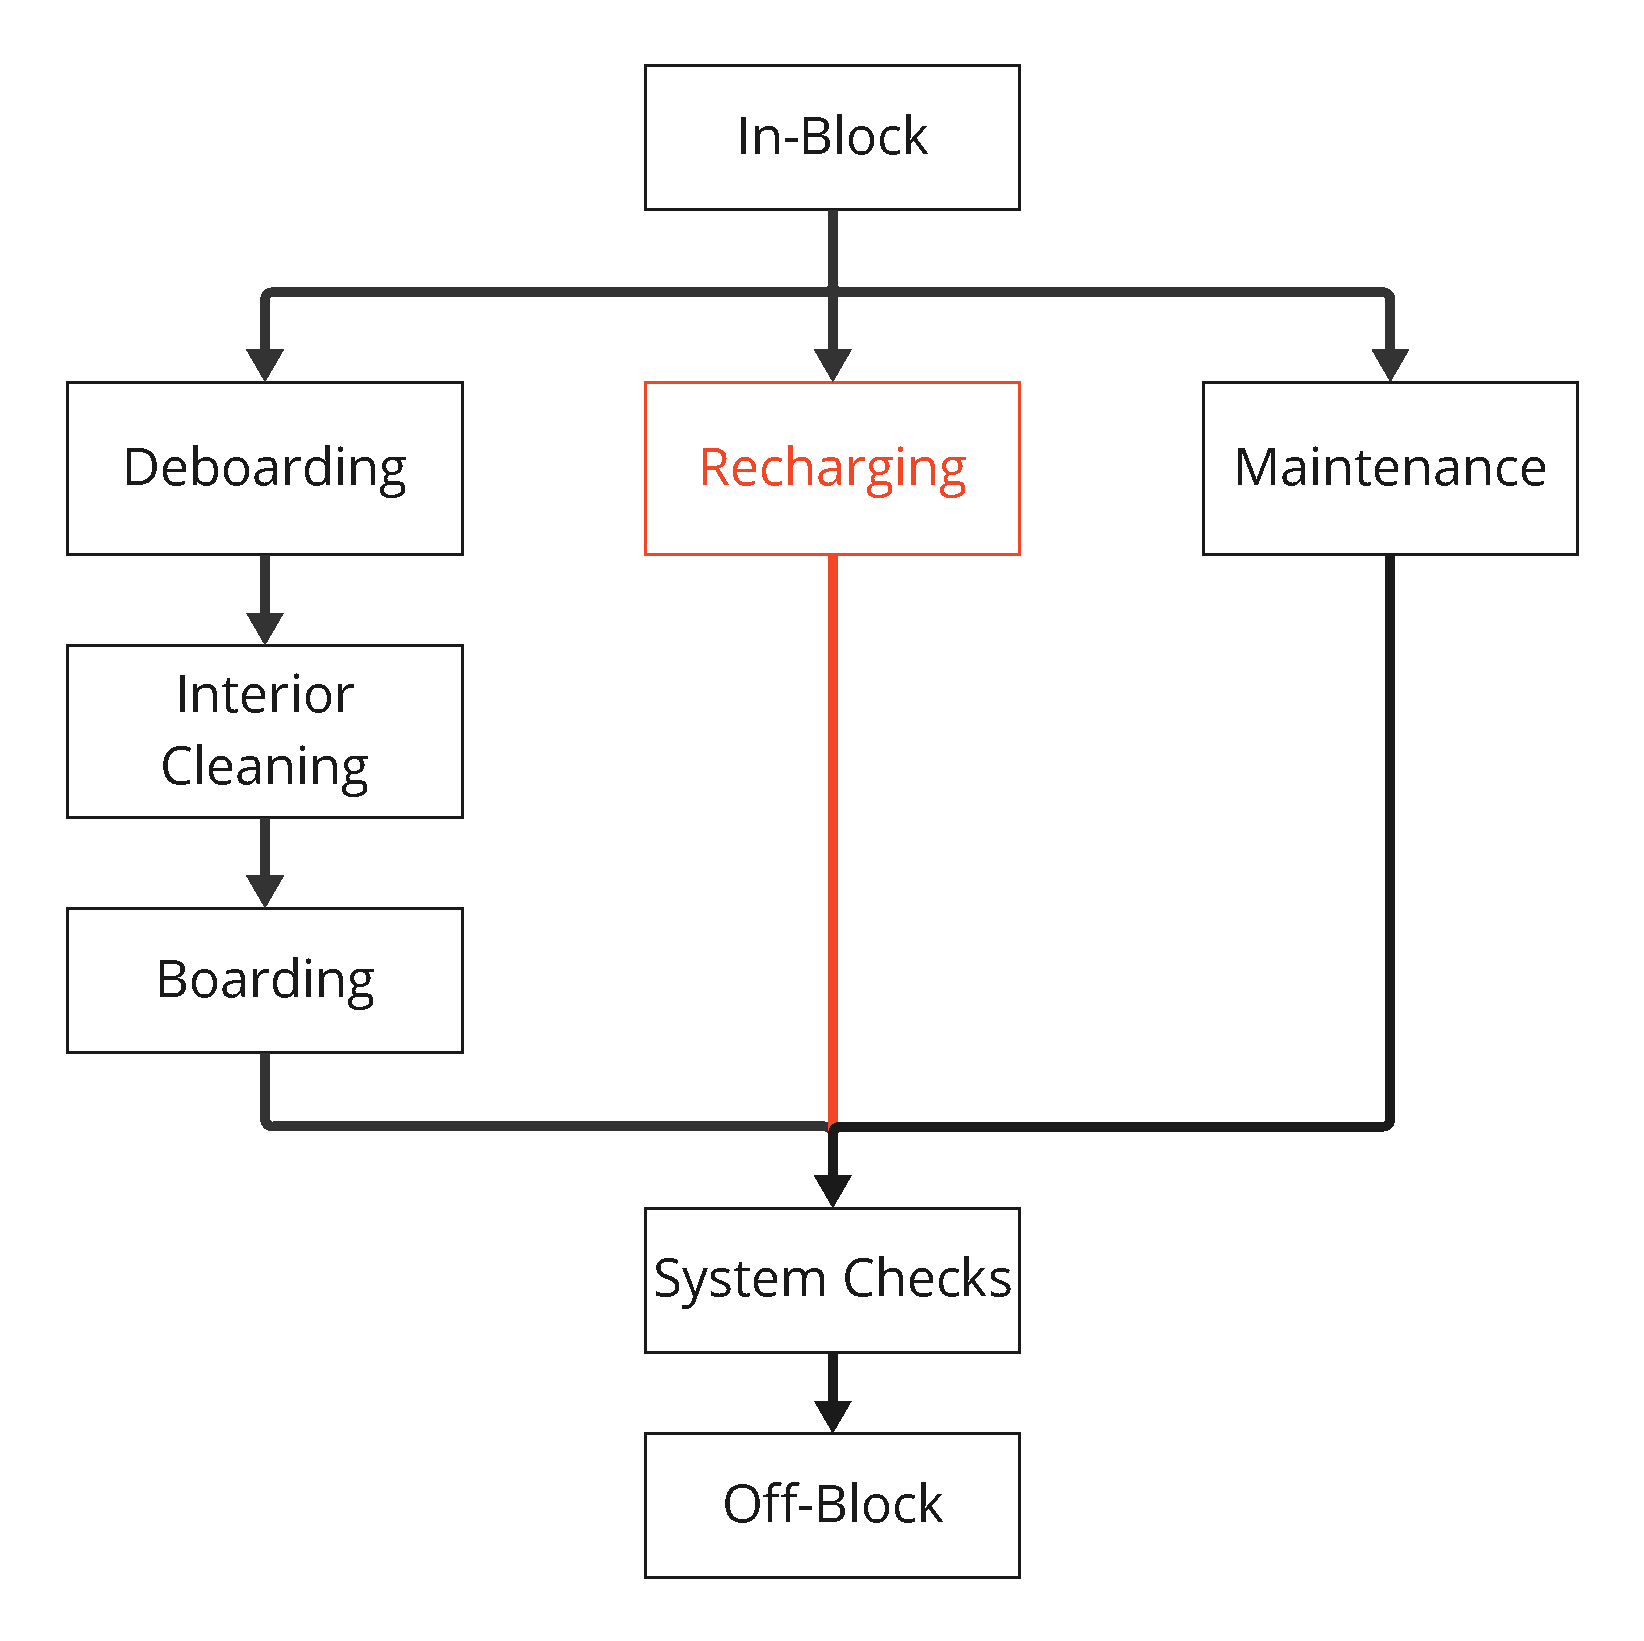
\includegraphics[width=.4\textwidth]{figures/Market Analysis/block_landing}
    \caption{Turnaround diagram \textit{Swing} including the expected critical path}
    \label{fig:block_turnaround}
\end{figure}

\begin{figure}[!htpb]
    \centering
    \rotatebox{270}{%
    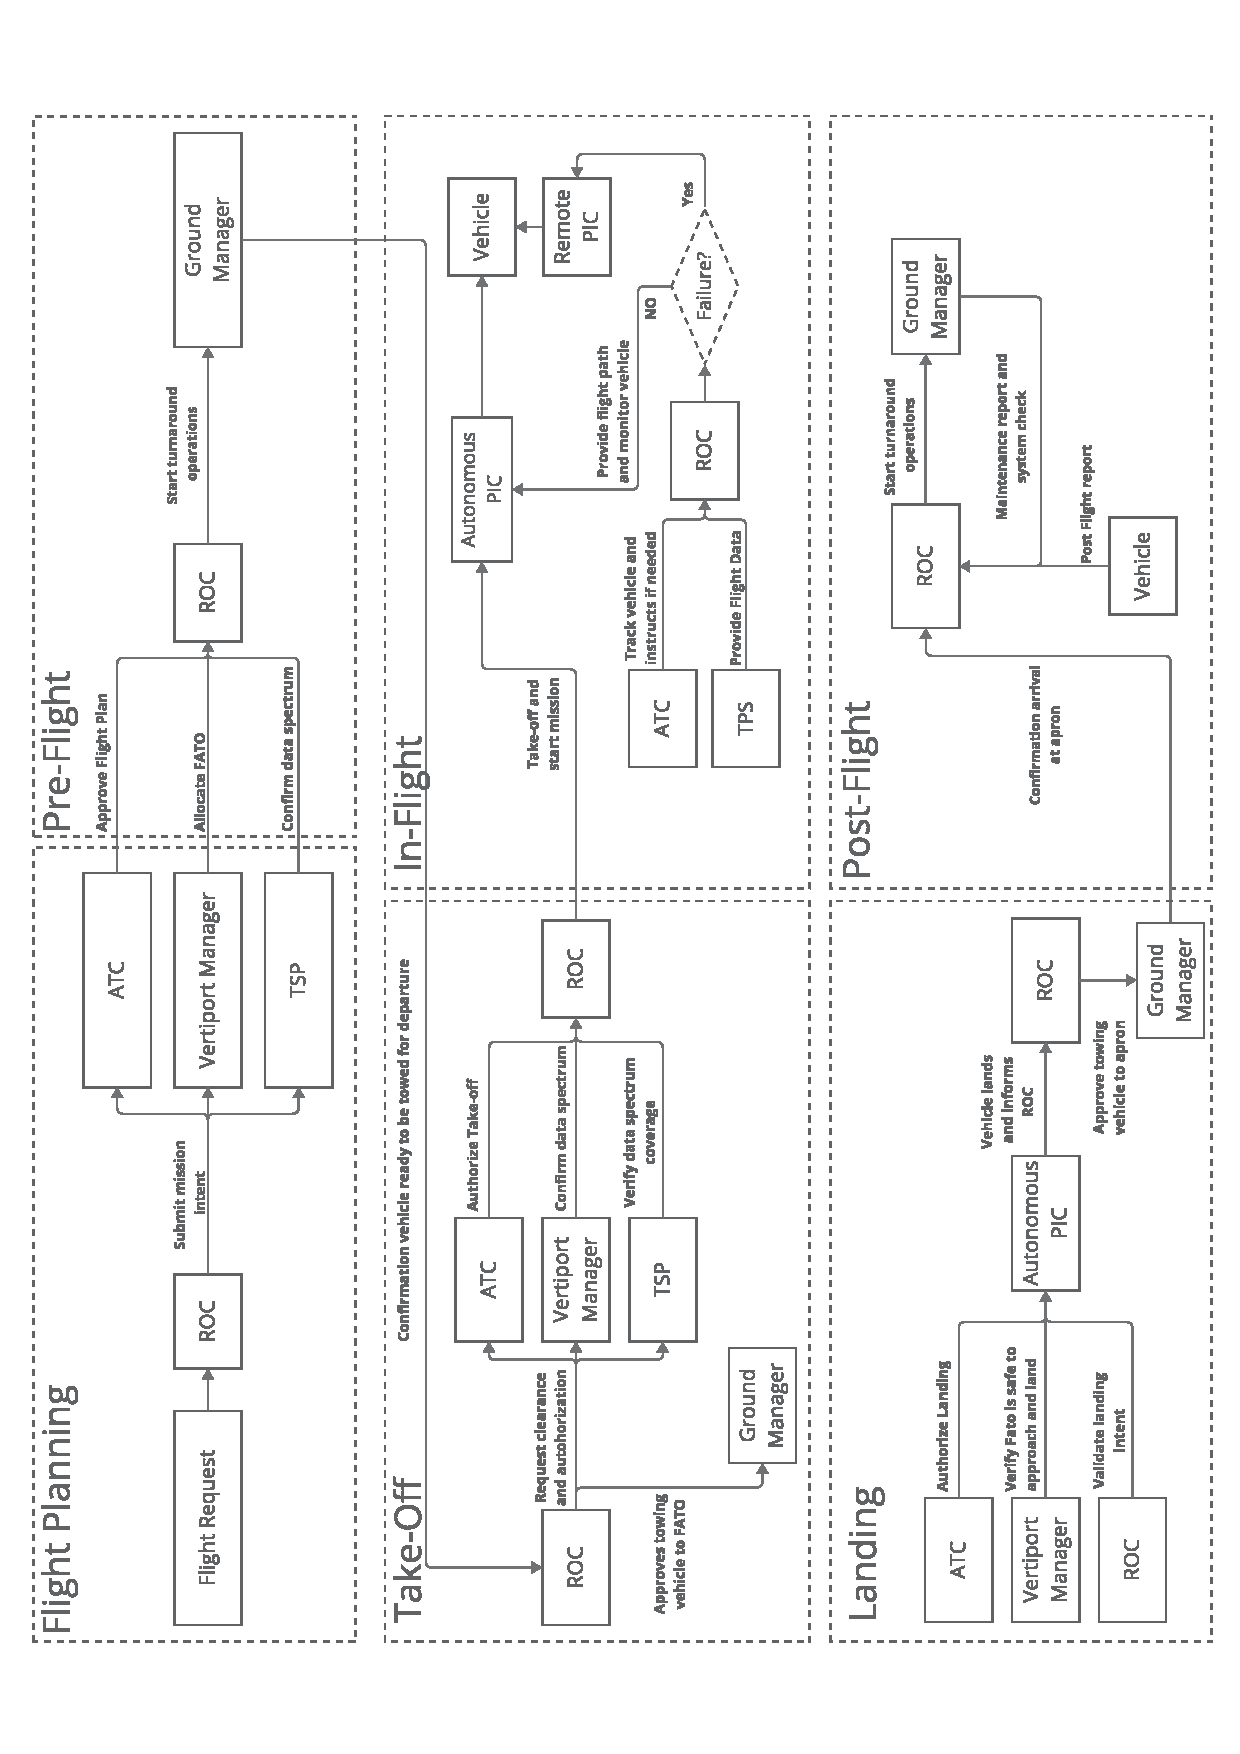
\includegraphics[width=.8\textwidth]{figures/Market Analysis/logistic diagram}
    }
    \caption{Operation diagram \textit{Swing}}
    \label{fig:log_diag}
\end{figure}

\subsubsection{Maintenance}
Besides the regular quick inspections during post-flight operations, a more extensive inspection has to be performed on the \textit{Swing}.

All subsystems are visually, mechanically, and electrically inspected during this inspection. 
The hinge, especially, should have regular inspection and maintenance since it must withstand high loads and is a critical subsystem. 
The subsystems bought from other companies, such as the electric motors, will be inspected by the designated company.

The vehicle must adhere to the regulations set by EASA, because EASA provides the Airworthiness Readiness Certificate (ARC) for aviation in Europe.
The eVTOL needs to comply with EASA’s continuing airworthiness requirements, which include regular maintenance, inspection and updates to the aircraft.
An approved Part M Continuing Airworthiness Management Organisation (CAMO) issues these ARC’s, which are often valid for one year.
Therefore, constant and extensive maintenance should be conducted and the Aircraft Maintenance Program (AMP) should be updated~\cite{easa_part_m_syllabus_2021}.


\subsubsection{Storage}
The vehicles are stored or placed on standby in the vertihubs and vertibases. 
The benefit of the \textit{Swing}, with its reduced ground footprint of four parking spaces due to the rotating wings, is that it can be stored easily. 
The vehicles will be charged during storage, so the vehicle battery is charged when deployed.
To release the constant bending moment on the hinge the wings will be supported by a wing support strut during storage.
This decreases the fatigue on the hinge and increases the reliability and safety of the vehicle.


\subsection{Downwash Protection Area}
One of the main operational concerns of vertiports are the huge downwash speeds created by eVTOLs, which need to be carefully managed.
\Cref{fig:max_downwash} shows the maximum downwash speeds per area that EASA established \cite{easa2022vertiports}, based on the CASA regulations, which differ quite a bit per type of area.
Hence, the vertiport must account for a so-called downwash protection area, in order to realise safe operations and logistics.
This protection area is meant to prevent injury to passengers, personnel, and affected public, but also damage to vertiports, buildings, vehicles, and utilities.


\subsection{Autonomous Flight}
Due to the autonomous system onboard of the \textit{Swing eVTOL}, the vertiport configuration can vastly differ from the classical heliport style.
In particular, the current lighting guidance is mostly based on pilot guidance, historical measures, and overseas regulations, which would not be needed for autonomous eVTOLs.
Think of the possibilities of integrated LEDs that can change the size and shapes of markings, or even QR codes that help the eVTOL approach or send important information about landing conditions \cite{CASA2024vertiports}.
This is further illustrated by \Cref{fig:vertiport_futuristic}, showing only some of the wide array of possibilities.

\begin{minipage}{0.62\linewidth}
    \begin{figure}[H]
    \centering
    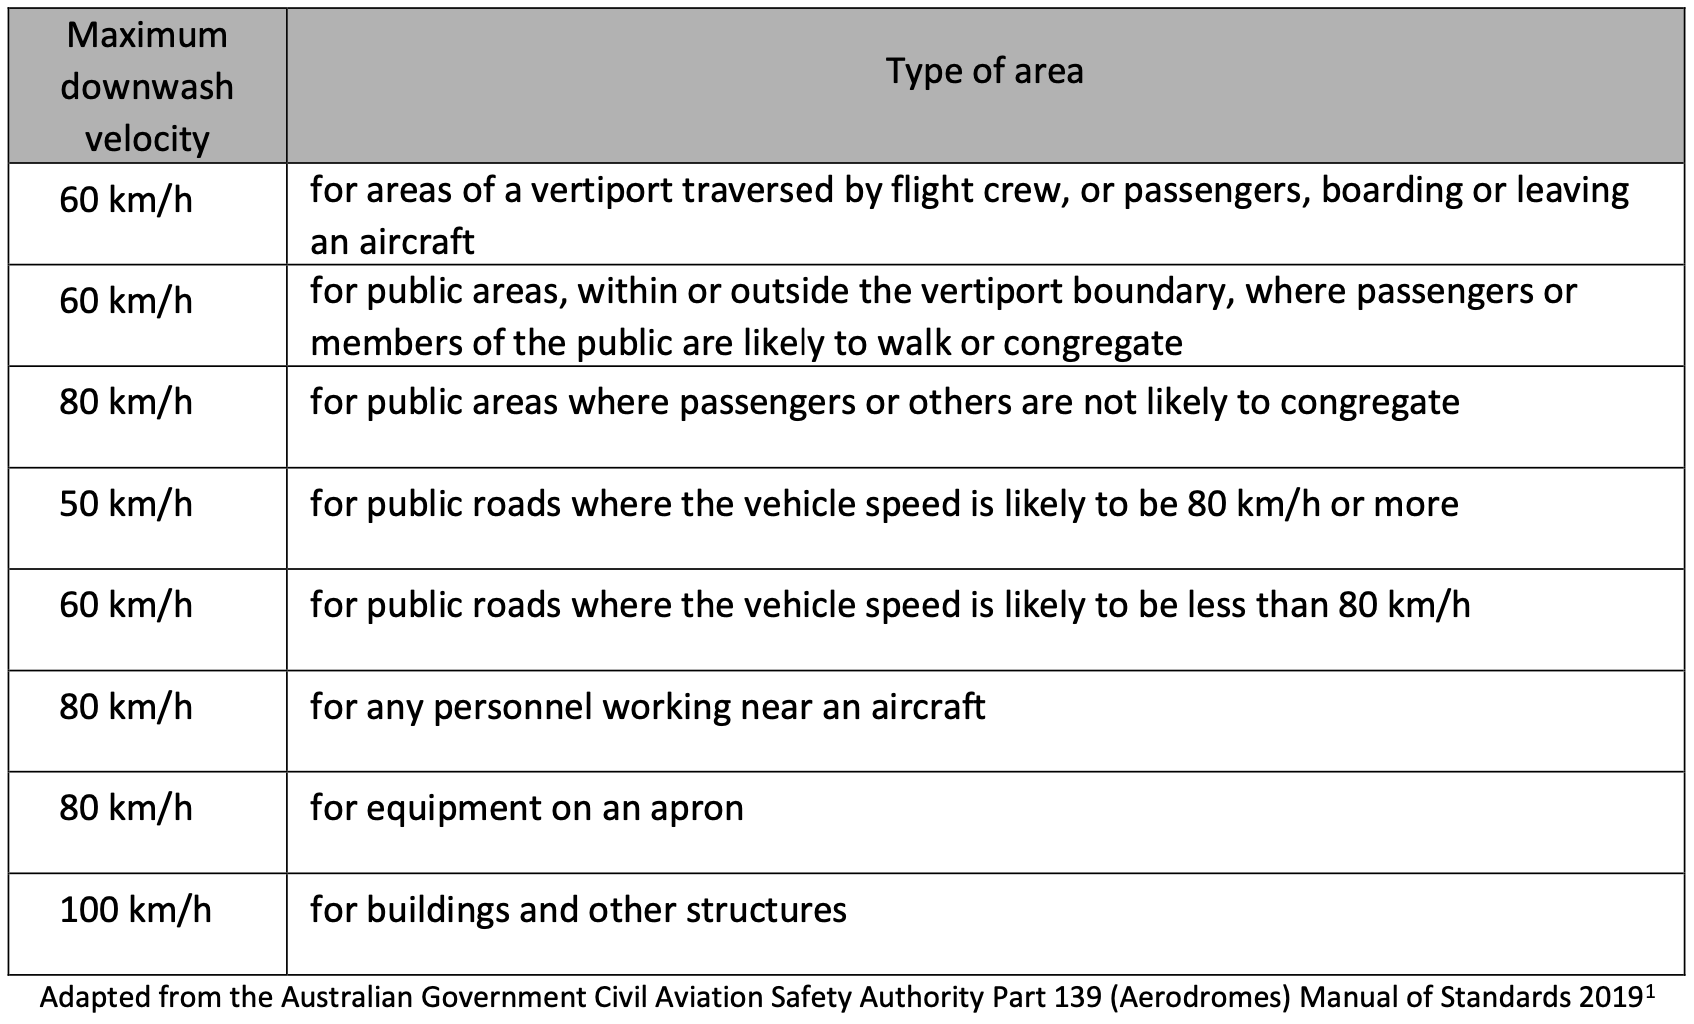
\includegraphics[width=1\linewidth]{figures/maximum_downwash_speeds}
    \caption{Maximum downwash speeds \cite{easa2022vertiports}}
    \label{fig:max_downwash}
    \end{figure}
\end{minipage}
\begin{minipage}{0.38\linewidth}
    \begin{figure}[H]
    \centering
    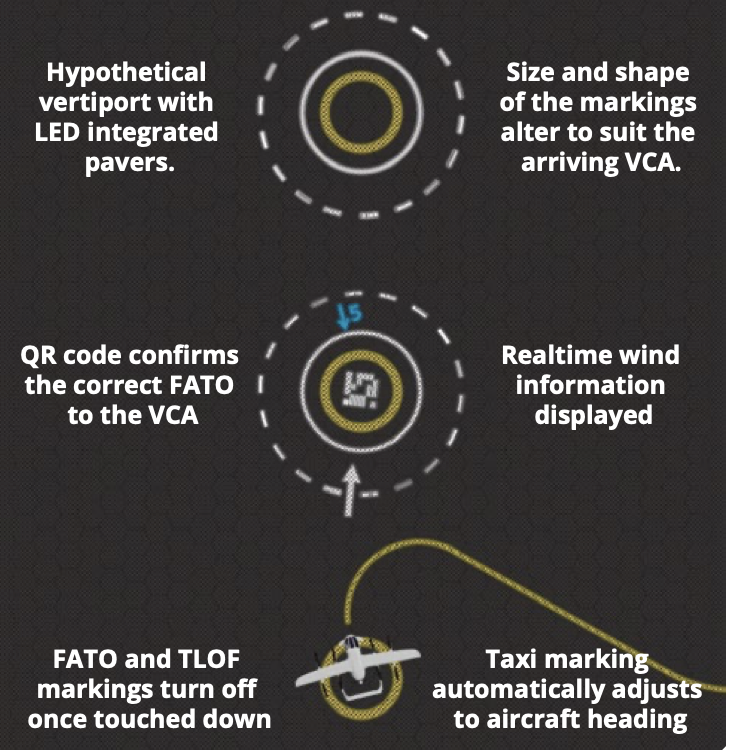
\includegraphics[width=1\linewidth]{figures/Vertiport-futuristic}
    \caption{Vertiport possibilities \cite{CASA2024vertiports}}
    \label{fig:vertiport_futuristic}
    \end{figure}
\end{minipage}


\section{RAMS Analysis}
\label{sec:Reliability_Availability_Maintainability_and_Safety}
The design’s reliability, availability, maintainability and safety (RAMS) must be analysed to reduce the impact and occurrence of any failures during operation.
The market position of the vehicle will increase if the vehicle adheres to these constraints.

\subsubsection{Reliability}
The reliability quantifies how failure-free a system is during a predefined operational time.
It is crucial to express this numerically since it is important to the stakeholders’ needs and has to adhere to general testing guidelines.
The Failure Rate (FR) is a unit that represents this discipline.
Often the Mean Time Between Failure (MTBF), is used to express the reliability, however, the failure rate is more useful as this frequently appears in engineering and statistical calculations \cite{giovingo2019rams}.

The reliability can be estimated for the system and the subsystems based on parameters like the MTOW or partial weight of the subsystems, aircraft design role, sophistication level, complexity level, technological aircraft age and aircraft maintenance.

The estimation of the total failure rate of the system can be approached by the bottom-up or top-down method.
In the bottom-up method, the total failure rate of the system is the summation of each subsystem, as seen in \Cref{eq:fail_rate}, where $\lambda_{E_{i}}$ is the failure rate of the subsystem.

\begin{equation}
    \label{eq:fail_rate}
    \lambda = \sum_{i} \lambda_{E_{i}}
\end{equation}

The other approach is the top-down method, where the failure rate of the subsystem is obtained through the allocation of the system failure rate, which is defined on historical data. 

\begin{itemize}
    \item \textbf{Technological Age Index} (IA), is an index for the technology level used during the design process.
    \item \textbf{Complexity Index} (IC) indicates the aircraft’s complexity.
    \item \textbf{Role Index} (IR) states the importance of the role of the aircraft.
\end{itemize}
Using these definitions, the failure rate of the aircraft can be determined, seen in \Cref{eq:LambdaTopdown}.
Where \(\left( \frac{\lambda}{\text{MEW}} \right)_{\text{MCA}}\) is the failure rate divided by the Maximum Empty Weight (MEW) for Medium Civil Aircraft (MCA), and is assumed to be equal to \(\qty{1.8}{\frac{\text{failures}}{1000 \text{FH} \cdot t}}\) \cite{giovingo2019rams}.
Here, FH represents flight hours and \(t\) is time.

\begin{equation}
\label{eq:LambdaTopdown}
    \lambda = \left ( \frac{\lambda}{\text{MEW}} \right )_\text{MCA} \cdot \text{IR} \cdot \text{IC} \cdot \text{IA} \cdot \text{MEW}
\end{equation}

\begin{table}[H]
    \centering
    \begin{tabular}{cccc}
        \toprule
        \textbf{IA} & \textbf{IC} & \textbf{IR} & \textbf{MEW [kg]} \\
        \midrule
        0.6 & 1.4 & 1.0 & 1300 \\
        \midrule
        \multicolumn{4}{c}{} \\ % Empty row for better spacing
        \multicolumn{3}{r|}{\textbf{Total Failure Rate}} & \textbf{2.0} \\
        \bottomrule
    \end{tabular}
    \caption{Failure rate $\lambda$ of the vehicle}
    \label{tab:failure_rate}
\end{table}
The estimated failure rate for the system can be seen in \Cref{tab:failure_rate}.
 The subsystem weights were used as input together with historical data to estimate the failure rate, using \Cref{eq:li}.
Where lambda is the system failure rate, $K_{i}$ a normalised failure rate coefficient differing per subsystem that is obtained from historical data, $W_{i}\%$ the subsystem percentage weight and $\lambda_{i_{nn}}$ the non-normalised subsystem failure rate.
From historical data, the $K_{i}$ value is obtained \cite{giovingo2019rams} and the final result can be seen in \Cref{tab:subsystemfailurerate}.

\begin{equation}
\label{eq:li}
    \lambda_{i} = \lambda \frac{K_{i} W_{i}\%}{\sum_{i}\lambda_{i_{nn}}}
\end{equation}

\begin{table}[H]
\centering
\caption{Failure rate per subsystem top-down method}
\begin{tabular}{l|S[table-format=3.1]S[table-format=2]S[table-format=1.2]S[table-format=2]S[table-format=1.2]}
\toprule
\textbf{Subsystem} & \textbf{Mass [kg]} & \textbf{W [\%]} & \textbf{K$_i$} & \textbf{$\lambda_{i_{nn}}$} & \textbf{$\lambda_i$} \\ \hline

Structures & 580 & 47 & 0.07 & 3 & 0.04 \\ 
Propulsion & 184 & 15 & 1.59 & 24 & 0.30 \\ 
Battery & 400 & 32 & 3.04 & 98 & 1.24 \\ 
Other & 78.7 & 6 & 5.32 & 34 & 0.43 \\ \bottomrule
\end{tabular}
\label{tab:subsystemfailurerate}
\end{table}

Since the top-down method is used, the failure rate per subsystem sums to 2.0. A more extensive method should be used for further reliability analysis, where more subsystems and more accurate failure rates are included. 


\subsubsection{Safety}
The safety concerns to the state where the risk level of the design is acceptable and not exceeded.
It is related to the reliability of the design with a focus on catastrophic failures.
The Safety Failure Rate is the performance figure to assess safety.
Moreover, safety factors are included during the design process to omit the probability of catastrophic system failures.
The total system failure is estimated by \Cref{eq:safetyfailurerate}

\begin{equation}
    \label{eq:safetyfailurerate}
    \lambda_{S} = \frac{\lambda}{\text{RL}} < \lambda_{S_{\max}}
\end{equation}
Where $\lambda$ is equal to the failure rate and RL is the Role Index equal to \num{1e6} for civil aircraft~\cite{giovingo2019rams}.
The non-standardised safety failure rate $\lambda_{s_{i_{nn}}}$ of the $i_{th}$ subsystem is obtained using the following expression.
\begin{equation}
    \lambda_{s_{i_{nn}}} = \frac{\lambda_{i}}{\text{RL}\cdot(\text{RD})^2}\cdot \text{DC} \cdot \text{CR} \cdot \text{CP} \cdot \sqrt{\text{TC}}
\end{equation}
Where:
\begin{itemize}
    \item \textbf{Subsystem redundancy coefficient} (RD) takes the value of 1.7 in case of redundancy.
    \item \textbf{Subsystem duty cycle coefficient} (DC) expresses the ratio between the operation time of the subsystem and the aircraft life cycle, in terms of flight hours.
    It has a value between 0.1 and 1.
    \item \textbf{Subsystem criticality coefficient} (CR) takes a value smaller than one if the subsystem strongly influences aircraft safety and greater than one if the subsystem is not critical for aircraft safety.
    \item \textbf{Subsystem complexity coefficient} (CP) expresses the complexity of the subsystem.
    If the subsystem is complex, the value is greater than one; otherwise, it is equal to one.
    \item \textbf{subsystem technological sophistication coefficient} (TC) expresses the technological level and novelty of each subsystem and uses the same scale as IC.
\end{itemize}
The summation of all the safety failure rates of the aircraft subsystems has to be equal to the total safety failure rate, therefore, it has to be normalised as seen in \Cref{eq:safety_normalised}


\begin{equation}
    \label{eq:safety_normalised}
    \lambda_{s_{i}} = \lambda_{s_{i_{nn}}} \frac{\lambda_{S}}{\sum_{i} \lambda_{S_{i_{nn}}}}
\end{equation}

The final values are put in \Cref{tab:safety_analysis}, where the coefficients are preliminary and estimated.
\begin{table}[H]
\caption{Safety failure rate}
\centering
\begin{tabular}{l|S[table-format=1.1]S[table-format=1.1]S[table-format=1.1]S[table-format=1.1]S[table-format=1.1]S[table-format=2.1]S[table-format=2.2]}
\toprule
\textbf{Subsystem} & \textbf{RD}  & \textbf{DC}  & \textbf{CR}  & \textbf{CP}  & \textbf{TC}  & \textbf{$\lambda_{S_{inn}}$ [\num[print-unity-mantissa=false]{1e-7}]} & \textbf{$\lambda_{S_i}$ [\num[print-unity-mantissa=false]{1e-7}]} \\ \midrule
Structures &1.7 & 1   & 0.8 & 1.2 & 1.3 & 1.6E-01 & 6.8E-01      \\
Propulsion &1.7 & 1   & 0.5 & 1.3 & 1.5 & 8.2E-01 & 3.6E-00      \\
Battery &1.7 & 1   & 0.6 & 1.1 & 1.1 & 3.0E-00 & 1.3E1      \\
Other &1.7 & 0.5 & 0.9 & 1   & 1   & 6.6E-01 & 2.9E-00     \\ \bottomrule
\end{tabular}
\label{tab:safety_analysis}
\end{table}
The safety failure rates must be validated to see if the order of magnitude is valid.
A paper by \textcite{safetyfailurerate} estimates the order of magnitude of failure rates for eVTOL and small general electric aircraft.
For different assessment levels,
the failure rate had a similar order of magnitude in the range of \numrange[print-unity-mantissa=false]{1e-6}{1e-9}.
There also has to be accounted for ground regulation safety.
During take-off and landing, there should be enough ground clearance and strict guidelines to mitigate the risk of accidents occurring, and therefore increase safety.
This is described in \Cref{sec:vertiport_logistic}, where the ground operation logistics are analysed.


\subsubsection{Maintainability}
Maintainability in aircraft design refers to the likelihood that an item will be kept in, or restored, to a specified condition within a given time frame, when appropriate and predefined procedures and resources are used \cite{conlon1982test}.
The Maintenance Man Hours per Flight (MMH/FH) is a commonly used maintainability performance figure, which divides the labour hours spent on maintenance by the flight hours during that period and is estimated, on system level, using the following relation in \Cref{eq:MMHFH}.

\begin{equation}
    \label{eq:MMHFH}
    \frac{\text{MMH}}{\text{FH}} = \frac{1}{6} \text{IRM} \cdot \text{CDTM} \cdot \text{IC} \cdot \text{IA} \cdot \text{MEW}^{0.25}
\end{equation}

Where IRM is the Maintenance Role Index, which is equal to 1.5 for civil aircraft and CDTM the Design to Maintain Coefficient that is dependent on the total attention paid to the maintenance, during the design process.
CDTM can be estimated by historical data, following from \textcite{giovingo2019rams}, which estimates the coefficient value based on the level of maintenance performed.
From this paper, the third level (RAMS discipline considered in design requirements) was chosen, which had a value of 1.2. The paper estimates the fraction 1/6 to account for the better technology that is available and the fact that the way of performing maintenance has changed.

The system value for the $\frac{\text{MMH}}{\text{FH}}= 0.3$, which is a preliminary value and has to be verified and validated.
An analysis conducted by \textcite{sieb2023identifying}, provided values ranging from 0.38 to 0.44 MMH/FH, which is in the same range.
However, the complex transwing mechanism is novel and, therefore, requires extensive maintenance.
This also accounts for the electric propulsion and V-tail configuration.
Therefore, a more intensive subsystem analysis has to be conducted to estimate a better MMH/FH.

\subsubsection{Availability}
Availability translates the maintainability and system reliability characteristics into an index of effectiveness.
If both the characteristics have a high value, then the availability will be high consequently.
The vehicle ought to have high availability because it has to adhere to requirement Te-2-STK07-5, stating that the vehicle has to be operational for 345 days per year.
This includes weather conditions, according to requirement Te-2-STK07-5-2, stating the vehicle shall be able to withstand winds of up to 7 Beaufort.
Moreover, since the goal is to maximise the number of trips, the turnover time is kept as low as possible.